
% =========================================================================================
% HOMEWORK TEMPLATE %===================================================================
% =========================================================================================

% =========================================================================================
% LaTeX SETUP %============================================================================
% =========================================================================================
\documentclass{report}						% Change "article" to "report" to get rid of page number on title page
\usepackage{amsmath,amsfonts,amsthm,amssymb,empheq}
\usepackage{setspace}
\usepackage{Tabbing}
\usepackage{fancyhdr}
\usepackage{lastpage}
\usepackage{extramarks}
\usepackage{chngpage}
\usepackage{soul,color}
\usepackage{graphicx,float,wrapfig}
\usepackage[retainorgcmds]{IEEEtrantools}

% =========================================================================================
% TikZ SETUP %==============================================================================
% =========================================================================================
\usepackage{tikz}
\usepackage{verbatim}
\usetikzlibrary{shapes,arrows,positioning,calc,scopes,angles,quotes}
\usetikzlibrary{decorations.markings}

% =========================================================================================
% MARGINS %===============================================================================
% =========================================================================================
\topmargin=-0.45in      
\evensidemargin=0in     
\oddsidemargin=0in      
\textwidth=6.5in        
\textheight=9.0in       
\headsep=0.25in         

% =========================================================================================
% ASSIGNMENT INFORMATION %===============================================================
% =========================================================================================
\newcommand{\hmwkTitle}{Midterm Exam\ 1}
\newcommand{\hmwkDueDate}{ March\ 2,\ 2016}
\newcommand{\hmwkClass}{EE\ 324}
\newcommand{\hmwkClassTime}{Munk}
\newcommand{\hmwkClassInstructor}{Prof. Jens}
\newcommand{\hmwkAuthorName}{Blair Munro}

% =========================================================================================
% HEADER & FOOTER %=======================================================================
% =========================================================================================
\pagestyle{fancy}                                                       
\lhead{\hmwkAuthorName}                                                 
\chead{\hmwkClass\ (\hmwkClassInstructor\ \hmwkClassTime): \hmwkTitle}  
\rhead{\firstxmark}                                                     
\lfoot{\lastxmark}                                                      
\cfoot{}                                                                
\rfoot{Page\ \thepage\ of\ \pageref{LastPage}}                          
\renewcommand\headrulewidth{0.4pt}                                      
\renewcommand\footrulewidth{0.4pt}                                      

% =========================================================================================
% CUSTOM MATH COMMANDS %================================================================
% =========================================================================================
\newcommand{\ud}{\,\mathrm{d}}						%creates roman-script differential d , with added space
\newcommand{\pd}[2]{\frac {\partial #1}{\partial #2}} 										%partial derivative
\newcommand{\td}[2]{\frac {\mathrm{d} #1}{\mathrm{d} #2}}									  %derivative
\newcommand{\tdd}[2]{\frac {\mathrm{d}^2 #1}{\mathrm{d} #2^2}}  						      %second derivative
\newcommand{\val}[2]{#1 \text{ #2}}							 	    %formats a numerical value with text units
\newcommand{\comm}[1]{\qquad\text{#1}}
% =========================================================================================
% MAKE TITLE %=============================================================================
% =========================================================================================
\title{\vspace{2in}\textmd{\textbf{\hmwkClass:\ \hmwkTitle}}\\\normalsize\vspace{0.1in}\small{Due\ on\hmwkDueDate}\\\vspace{0.1in}\large{\textit{\hmwkClassInstructor\ \hmwkClassTime}}\vspace{3in}}
\date{}
\author{\textbf{\hmwkAuthorName}}

% =========================================================================================
% BEGIN DOCUMENT %=======================================================================
% =========================================================================================
\begin{document}
\begin{spacing}{1.1}
\maketitle

\newpage
\begin{enumerate}
%PROBLEMS ================================================================================
%	1
\item[{\bf \large 1.}] 
As depicted in Figure 1, there is a perfectly conducting track with a resistive sliding bar resting across the two rails. At $t=0$, a switch closes across the DC voltage source shown to complete the circuit. Current flows, and a force results, as given by the familiar \[\mathbf{F}=I\mathbf{\ell}\times\mathbf{B}.\]
This causes the bar to accelerate rightward.

Now as the bar speeds up from rest, so too does the magnetic flux through the loop change from zero to non-zero. By Lenz' Law, this induces a current in the circuit that creates B-field change in opposition to the prevailing trend, thus the induced current begins to slow the rate of acceleration down to zero. Where is this equilibrium point?

For the constant B-field given in the figure, determine the velocity of the bar as $t\to \infty$, in terms of $V_0$, $B_0$, and $\ell$.
\begin{figure}[!hbp]
\centering
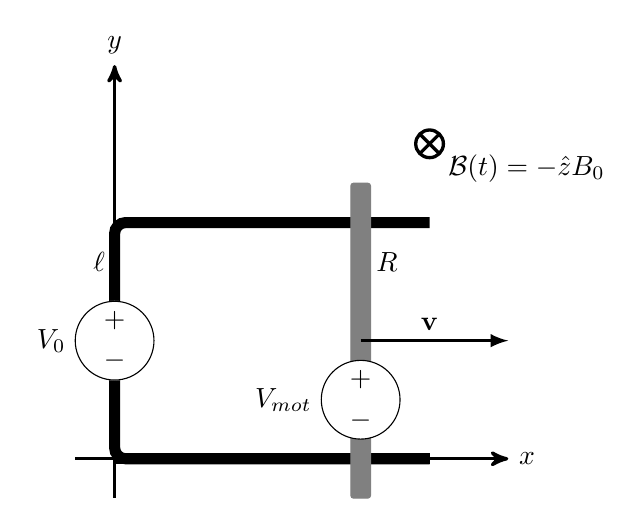
\begin{tikzpicture}[
	scale=1,
	vector/.style={very thick,->, >=latex},
	axis/.style={very thick, ->, >=stealth'}]
	\coordinate (O) at (0,0);
	\draw[axis] (O)--(0:5)node(X)[right]{$x$};
	\draw[axis] (O)--(90:5)node(Y)[above]{$y$};
	\draw[very thick] (O)--(180:0.5);
	\draw[very thick] (O)--(-90:0.5);
	\draw[line width=4pt,rounded corners=4pt] (4,0)--(O)|-(4,3);
	\draw[line width=4pt] (O)--(4,0);
	\filldraw[gray,rounded corners=1pt] (3,-0.5)coordinate(A) rectangle (3.25,3.5)coordinate(B);
	\filldraw[white] (0,1.5) circle (0.5cm);
	\draw (0,1.5) circle (0.5cm);
	\draw (0,2) node[below]{$+$};
	\draw (0,1) node[above]{$-$};
\begin{scope}[shift={(3+.25/2,-0.75)}]
	\draw[fill=white] (0,1.5) circle (0.5cm);
	\draw (0,2) node[below]{$+$};
	\draw (0,1) node[above]{$-$};
	\draw (-0.5,1.5) node[left]{$V_{mot}$};
\end{scope}
	\draw (-0.5,1.5) node[left]{$V_0$};
	\path(A)--(B)coordinate[pos=0.5](V);
	\draw[vector] (V)--(5,1.5); 
	\draw(4,1.5) node[above]{$\mathbf{v}$};
	\draw (3.2,2.5) node[right]{$R$};
	\draw (0,2.5) node[left]{$\ell$};
	\draw[shift={(4,4)},very thick,fill=white] (0,0)circle(5pt) (0.1,0)node[below right]{$\mathcal{B}(t)=-\hat z B_0$}; 
	\draw[shift={(4,4)},very thick] (0,0)--(-45:5pt) (0,0)--(45:5pt) (0,0)--(135:5pt) (0,0)--(-135:5pt);
\end{tikzpicture}
\caption{The ol' sliding bar trick.}
\end{figure}

\begin{IEEEeqnarray*}{lrCl}
\comm{at $t\to\infty$}&V_0&=&V_{mot}\\
&&=&\oint_C(\mathbf{v}\times\mathcal{B})\cdot \ud \mathbf{\ell}\\
&&=&\ell B_0 v \hat v\\
\end{IEEEeqnarray*}
I think it could be easy to overthink things at this point, and I am trying to avoid this if at all possible: I will insist to myself hoever, that I can rest easy by my sanity check concluding that the bar's resistance has no bearing on the final speed attained. For example, if R were very large, it acceleration due to $\mathbf{F}$ would be very small, but in the limit should still be the same velocity.

\[\boxed{v\to\frac{V_o}{\ell B_0}\text{ as }t\to\infty}\]
\newpage
%	2 
\item[{\bf \large 2.}]
Once upon a time, there was a linearly polarized uniform plane wave propagating through the ocean in the $+z$-direction. The seawater has the following characteristics: $\epsilon_r=80$, $\mu_r=1$, $\sigma=4$ S/m.
At a particular point---call it $z=0$---the electric field of the wave has an intensity given by \[\mathcal{E}(t)=\hat x 10\sin (2\pi\times 10^6t-\pi/8).\]
\begin{figure}[!hbp]
\centering
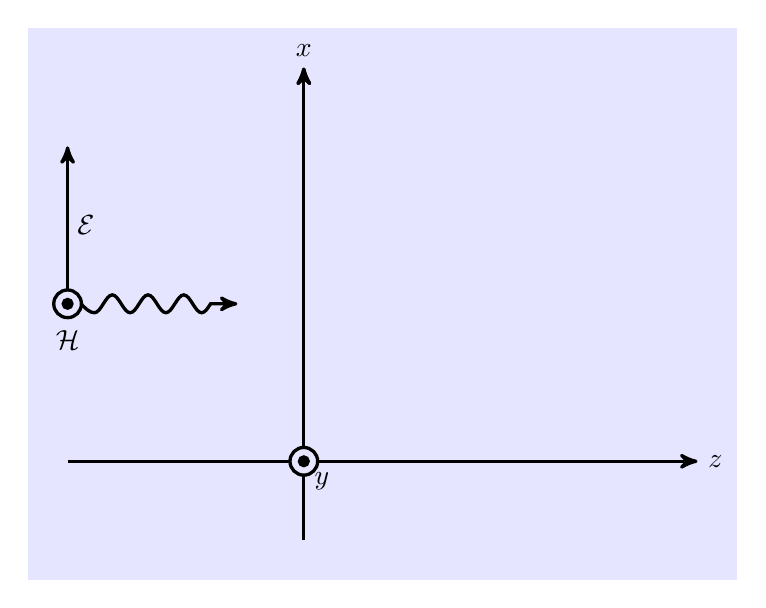
\begin{tikzpicture}[
	scale=1,
	vector/.style={very thick,->, >=latex},
	axis/.style={very thick, ->, >=stealth'}]
	\filldraw[blue!10] (-3.5,-1.5) rectangle (5.5,5.5);
	\draw[axis] (-180:3)--(0:5)node[right]{$z$};
	\draw[axis] (0,-1)--(90:5);
	\draw[axis] (90:5)node[above]{$x$};
	\draw[very thick,fill=blue!10] (0,0)circle(5pt) (0,0)node[below right]{$y$}; 
	\draw[fill=black] (0,0)circle(2pt);
	\draw[shift={(-3,2)},axis,x=0.75ex,y=0.75ex] (1.5,0) sin (3,-1) cos (4,0)sin (5,1) cos (6,0) sin (7,-1) cos (8,0)sin (9,1) cos (10,0) sin (11,-1) cos (12,0)sin (13,1) cos (14,0) sin (15,-1) cos (16,0)--(19,0);
	\draw[shift={(-3,2)},axis] (0,0)--(90:2);
	\draw[shift={(-3,2)}] (0,1) node [right]{$\mathcal{E}$};
	\draw[shift={(-3,2)},very thick,fill=blue!10] (0,0)circle(5pt) (0,-0.2)node[below]{$\mathcal{H}$}; 
	\draw[shift={(-3,2)},fill=black] (0,0)circle(2pt);
	
\end{tikzpicture}
\caption{Drowning in the waves.}
\end{figure}
\subitem{\bf\large (a)} Determine the attenuation constant $\alpha$, the phase constant $\beta$, the intrinsic impedance $\eta$, the phase velocity, and the wavelength.

First, by inspection of $\mathcal{E}(t)$ we need to recognize that $\omega=2\times10^6$ rad/s.

(Also recall that $\epsilon_0=8.854\times 10^{-12}$F/m, and $\mu_0=4\pi\times10^{-7}$H/m.)

\begin{IEEEeqnarray*}{lrCl}
\comm{we know the propagation constant,}&k&=&\omega\sqrt{\epsilon_r\mu_r}\sqrt{\epsilon_0\mu_0}\sqrt{1-j\frac{\sigma}{\omega\epsilon_r\epsilon_0}}\\
&\omega\sqrt{\frac{\mu\epsilon}{2}}&\approx& 0.0596\\
&\sqrt{1+\left(\frac{\sigma}{\omega\epsilon}\right)^2}&\approx&2823.58\\
&\alpha &=&\omega\sqrt{\frac{\mu\epsilon}{2}}\left[\sqrt{1+\left(\frac{\sigma}{\omega\epsilon}\right)^2}-1\right]^{1/2}\\
&\left[\sqrt{1+\left(\frac{\sigma}{\omega\epsilon}\right)^2}-1\right]^{1/2}&\approx &53.128\\
&\beta &=&\omega\sqrt{\frac{\mu\epsilon}{2}}\left[\sqrt{1+\left(\frac{\sigma}{\omega\epsilon}\right)^2}+1\right]^{1/2}\\
&\left[\sqrt{1+\left(\frac{\sigma}{\omega\epsilon}\right)^2}+1\right]^{1/2}&\approx& 53.147\\
\end{IEEEeqnarray*}

\begin{IEEEeqnarray*}{lrCl}
&\eta=\frac{\omega\mu}{k}&=& \sqrt{\frac{\mu}{\epsilon}}\left(1-j\frac{\sigma}{\omega\epsilon}\right)^{-1/2}\\
&\sqrt{\frac{\mu}{\epsilon}}=j9.204\times 10^4 &&\\
&\left(1-j\frac{\sigma}{\omega\epsilon}\right)^{-1/2} =2.297\times 10^{-06} + j2.297\times 10^{-06}&&\\
\end{IEEEeqnarray*}
Phase velocity $ v_p=\frac{\omega}{\beta}$, and the wavelength is $\lambda f = \frac{c}{\sqrt{\epsilon_r\mu_r}}$
\[\boxed{\beta=53.147\qquad\alpha=53.128}\]
\[\boxed{\eta=-0.2114 + j0.2114}\]
\[\boxed{v_p = 1.822\times 10^5 m/s \qquad \lambda = 5.34 m}\]

\subitem{\bf\large (b)} Find the distance that this lonely wave must travel for its magnitude of $\mathbf{E}$ to decay to 0.01 V/m.
\begin{IEEEeqnarray*}{lrCl}
&\mathcal{E}(t)&=&\hat x 10 e^{-53.128 z}\cos(2\pi\times 10^6 -53.147z+3\pi/8)\\
\comm{we want to find where}\qquad & \frac{1}{e^{-\alpha d}} &=& 1000\\
&e^{\alpha d}&=&1000\\
&d&=&\frac{\ln(1000)}{\alpha}\\
\end{IEEEeqnarray*}

\[\boxed{d = 0.13 m}\]  murky water. (or Im wrong.)
\subitem{\bf\large (c)} Write expressions for $\mathcal{E}(z,t)$ and $\mathcal{H}(z,t)$.
\[\boxed{\mathcal{E}(z,t)=\hat x10e^{-53.127z}\cos(2\pi\times10^6 t -53.147z+3\pi/8)}\]
$\mathcal{H}(z,t)=\hat y \frac{10}{-23.65 -j23.65}\cos(2\pi\times10^6 t -53.147z+3\pi/8)$
$\mathcal{H}(z,t)=\hat y 0.4228 e^j2.3564 e^{-53.127z}\cos(2\pi\times10^6 t -53.147z+1.178)$
\[\boxed{\mathcal{H}(z,t)=\hat y 0.4228 e^{-53.127z}\cos(2\pi\times10^6 t -53.147z+3.53)}\]
\newpage
\item[{\bf \large 3.}]
Consider a uniform plane-wave in free space $(\mu=\mu_0, \epsilon=\epsilon_0)$, incident to a layered slab of dielectric material. The first layer has thickness $d$ with permittivity $\epsilon_2$, and the second layer extends forever with permittivity $\epsilon_3$. Assume $\mu=\mu_0$ throughout. I am also going to assume this is the problem that was missing a frequency: let it be $f=200MHz$.
\begin{figure}[!hbp]
\centering
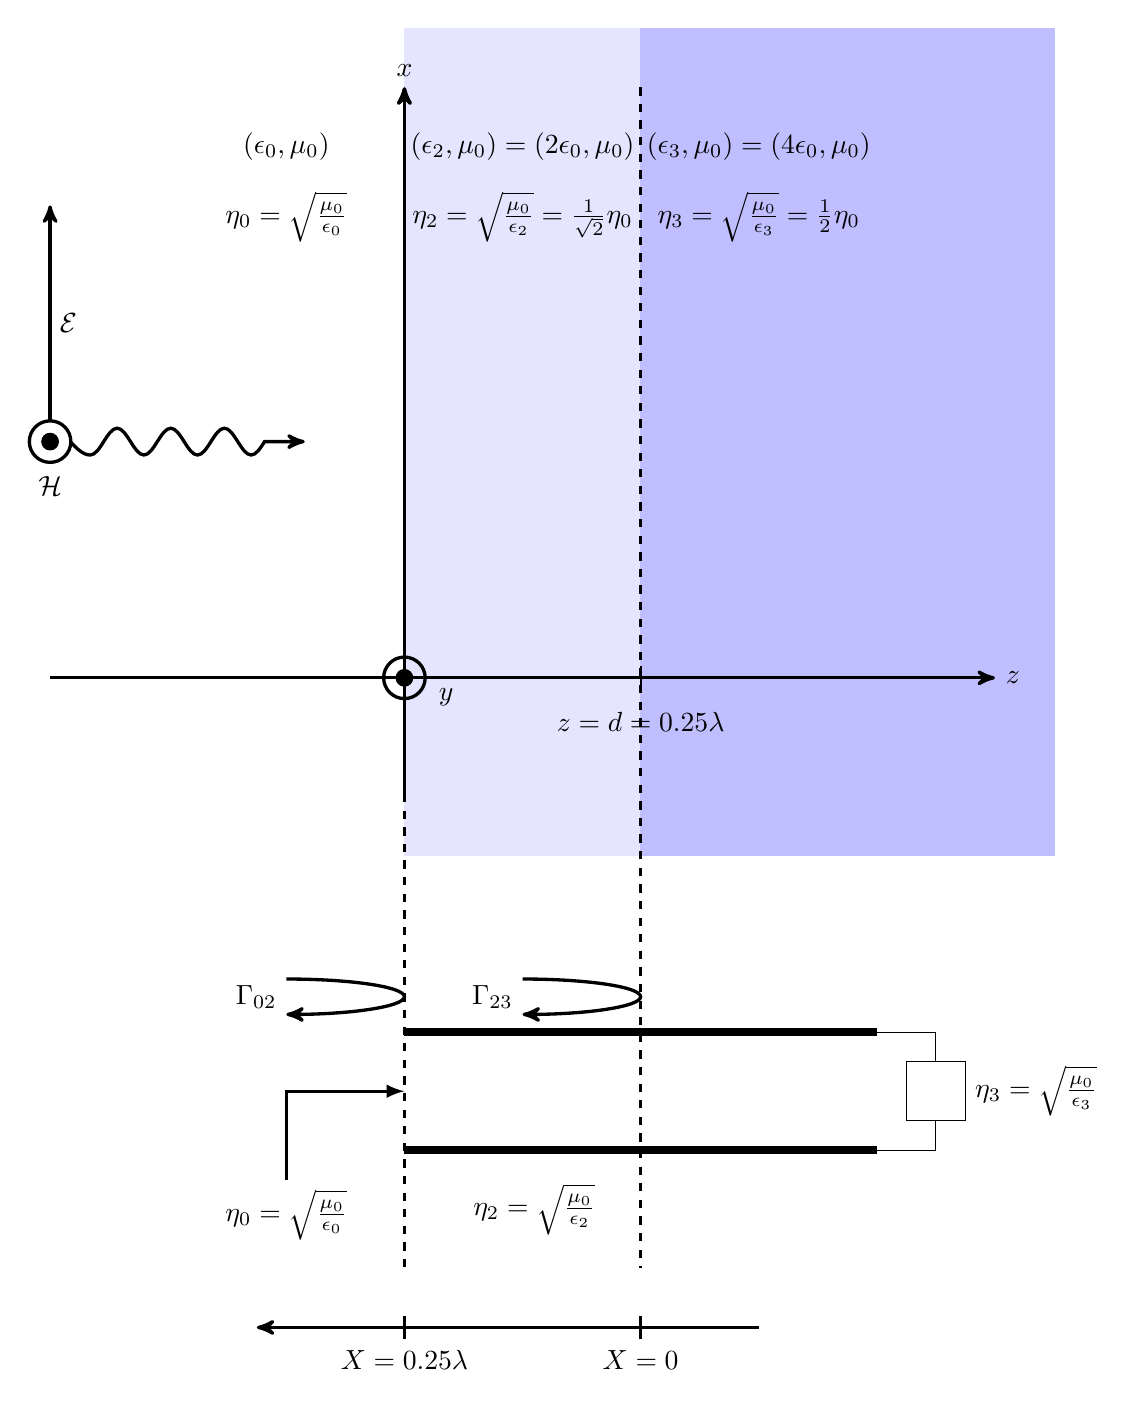
\begin{tikzpicture}[
	scale=1.5,
	vector/.style={very thick,->, >=latex},
	axis/.style={very thick, ->, >=stealth'}]
	\filldraw[blue!10] (0,-1.5) rectangle (2,5.5);
	\filldraw[blue!25] (2,-1.5) rectangle (5.5,5.5);
	\draw[axis] (-180:3)--(0:5)node[right]{$z$};
	\draw[axis] (0,-1)--(90:5);
	\draw[axis] (90:5)node[above]{$x$};
	\draw[very thick,dashed] (0,0)--(-90:5);
	\draw[very thick,dashed] (2,5)--(2,-5);
	\draw[very thick] (0,0)circle(5pt) (.2,0)node[below right]{$y$}; 
	\draw[fill=black] (0,0)circle(2pt);
	\draw[shift={(-3,2)},axis,x=0.75ex,y=0.75ex] (1.5,0) sin (3,-1) cos (4,0)sin (5,1) cos (6,0) sin (7,-1) cos (8,0)sin (9,1) cos (10,0) sin (11,-1) cos (12,0)sin (13,1) cos (14,0) sin (15,-1) cos (16,0)--(19,0);
	\draw[shift={(-3,2)},axis] (0,0)--(90:2);
	\draw[shift={(-3,2)}] (0,1) node [right]{$\mathcal{E}$};
	\draw[shift={(-3,2)},very thick,fill=white] (0,0)circle(5pt) (0,-0.2)node[below]{$\mathcal{H}$}; 
	\draw[shift={(-3,2)},fill=black] (0,0)circle(2pt);
	\draw(1,4.5) node{$(\epsilon_2,\mu_0) =(2\epsilon_0,\mu_0)$} (3,4.5) node{$(\epsilon_3,\mu_0)=(4\epsilon_0,\mu_0)$} (-1,4.5) node{$(\epsilon_0,\mu_0)$};
	\draw[thick] (2,-0.1)--(2,.1) (2,-.2)node[below]{$z=d =0.25\lambda$};
	\draw(-1,3.9) node{$\eta_0=\sqrt{\frac{\mu_0}{\epsilon_0}}$} (3,3.9) node{$\eta_3=\sqrt{\frac{\mu_0}{\epsilon_3}}=\frac{1}{2}\eta_0$} (1,3.9) node{$\eta_2=\sqrt{\frac{\mu_0}{\epsilon_2}}=\frac{1}{\sqrt{2}}\eta_0$};
\draw[shift={(1,-2.7)},axis] (90:.15)arc(90:-90:1 and 0.15);
	\draw (1,-2.7) node[left]{$\Gamma_{23}$};
	\draw[shift={(-1,-2.7)},axis] (90:.15)arc(90:-90:1 and 0.15);
	\draw (-1,-2.7) node[left]{$\Gamma_{02}$};
		\begin{scope}[shift={(0,-4)}]
		\draw[line width=3pt] (0,1)--(4,1);
		\draw[line width=3pt] (0,0)--(4,0);
		\draw (4,1)--(4.5,1)--(4.5,0)--(4,0);
		\draw[fill=white] (4.25,0.75) rectangle (4.75,0.25);
		\draw (4.75,0.5) node[right]{$\eta_3=\sqrt{\frac{\mu_0}{\epsilon_3}}$};
		\draw (0.5,-.5) node[right]{$\eta_2=\sqrt{\frac{\mu_0}{\epsilon_2}}$};
		\draw[vector] (-1,-0.25)|-(0,0.5);
		\draw (-1,-0.25) node[below]{$\eta_0=\sqrt{\frac{\mu_0}{\epsilon_0}}$};
		\draw[axis](3,-1.5)--(-1.25,-1.5);
		\draw[very thick] (2,-1.4)--(2,-1.6)	node[below]{$X=0$};	
		\draw[very thick] (0,-1.4)--(0,-1.6)	node[below]{$X=0.25\lambda$};
		\end{scope}
\end{tikzpicture}
\caption{Double-Dielectrics and the Transmission line model equivalent.}
\end{figure}
\newpage
\subitem{\bf\large (a)} What is an expression for the reflection coefficient at $x=0$?
First, calculate reflection coefficient at the second interface.
\begin{IEEEeqnarray*}{rClr}
\Gamma_{23}&=&\frac{\eta_3-\eta_2}{\eta_3+\eta_2}	&\comm{However much  we have reflecting}\\
&=&\frac{\frac{1}{2}\eta_0-\frac{1}{\sqrt{2}}\eta_0}{\frac{1}{2}\eta_0+\frac{1}{\sqrt{2}}\eta_0}		&\comm{}\\
\Gamma_{23}&=&\frac{1-\sqrt{2}}{1+\sqrt{2}} \approx -0.172&\comm{}\\
&=&\frac{	\frac{1}{\sqrt{2}}-1}{	\frac{1}{\sqrt{2}}+1}&\\
\Gamma_{02}&=&\frac{	\sqrt{2}-2}{	\sqrt{2}-2}\approx -0.172&\\
\Gamma_(d)&=&\frac{\eta_2(1+\Gamma_{23}e^{-j2\beta d})-\eta_1(1-\Gamma_{23}e^{-j2\beta d})}{\eta_2(1+\Gamma_{23}e^{-j2\beta d})+\eta_1(1-\Gamma_{23}e^{-j2\beta d})}&\\
\Gamma_{02}&=&\frac{\eta_2-\eta_0}{\eta_2+\eta_0}&\\
\Gamma_{}&=&\frac{\Gamma_{02}+\Gamma_{23}e^{-j2\beta d}}{1+\Gamma_{02}\Gamma_{23}e^{-j2\beta d}}&\\
\end{IEEEeqnarray*}

\[\boxed{\Gamma_{23}=\frac{\Gamma_{02}+\Gamma_{23}e^{-j2\beta d}}{1+\Gamma_{02}\Gamma_{23}e^{-j2\beta d}}\approx \frac{-0.172-0.172e^{-j2\beta d}}{1+0.0296e^{-j2\beta d}}}\]zx

\subitem{\bf\large (b)} If $d=0.25\lambda$, what is the reflection coefficient in polar form at $x=0$.
\begin{IEEEeqnarray*}{rClr}
\beta&=&\frac{2\pi f}{c}\sqrt{\mu_r\epsilon_r}\\
&=&\frac{2\pi f}{c}\sqrt{\mu_r\epsilon_r}&\\
-j2\beta X &=&-j\frac{4\pi f}{c}\sqrt{\mu_r\epsilon_r}X&\\
X&=&\lambda/4&\\
\lambda f &=& c &\\
-j2\beta X\Bigl|_{X=\lambda/4}&=&-j\frac{4\pi f}{c}\sqrt{\mu_r\epsilon_r}\frac{\lambda}{4}&\\
&=&-j\frac{\pi c}{c}\sqrt{\mu_r\epsilon_r} = -j\pi\sqrt{\mu_r\epsilon_r} &\\
\Gamma(X)&=& \frac{1-1.41e^{-j 2\beta X}} {1+1.41e^{-j2\beta X}}&\\
\Gamma(X)\Bigl|_{X=\lambda/4}&=&\frac{1-1.41e^{-j\pi\sqrt{\mu_r\epsilon_r}}}{1+1.41e^{-j\pi\sqrt{\mu_r\epsilon_r}}}&\\
\pi\sqrt{\mu_r\epsilon_r}&\approx & 8.8858&\
\end{IEEEeqnarray*}

\[\boxed{\Gamma_{02}\approx -1.74+j2.55=3.09\angle124^\circ}\]
This is a nonsense answer. I will try to keep it under 1 next time.

\subitem{\bf\large (c)} Verify this result using a Smith Chart.

\begin{figure}[!hbp]
\centering
\begin{tikzpicture}[
	scale=1,
	vector/.style={very thick,->, >=latex},
	axis/.style={very thick, ->, >=stealth'}]
		%	SMITH CHART: 
		%	2.34pt/mm	210pt, outer-mid	201pt, outer-inmid	225pt, outer	192pt, inner	
		%	[thick](90:226pt)--(90:238pt)		
		\node[inner sep=0pt] (russell) at (0,0){\includegraphics[width=1\textwidth]{SMITHCHARTSCAN.jpg}};
		\end{tikzpicture}
\caption{Smith Chart}
\end{figure}
%	4
\item[{\bf \large 4.}]
Derive the following general expressions for the attenuation and phase constant $k=\beta-j\alpha$ for a conducting medium:
\[\alpha =\omega\sqrt{\frac{\mu\epsilon}{2}}\left[\sqrt{1+\left(\frac{\sigma}{\omega\epsilon}\right)^2}-1\right]^{1/2}\]
\[\beta =\omega\sqrt{\frac{\mu\epsilon}{2}}\left[\sqrt{1+\left(\frac{\sigma}{\omega\epsilon}\right)^2}+1\right]^{1/2}\]
After doing so, obtain expressions for the limiting cases wherein $\omega\to\infty$ and $\omega\to0$.
For lossy media, we express the propagation constant using \[k=\omega\sqrt{\mu\epsilon}\sqrt{1-j\frac{\sigma}{\omega\epsilon}}\equiv\ \beta-j\alpha\]
To determine alpha and beta, we need to find the real and imaginary part of a number which is the root of a complex quantity, to do so, we make our lives easier by simplifying notation with a change in variables:

\begin{IEEEeqnarray*}{lrCl}
&\omega\sqrt{\mu\epsilon}\sqrt{1-j\frac{\sigma}{\omega\epsilon}}&=& \beta-j\alpha\\
\comm{change variables, let}&(B+jA)^2&=&1-j\frac{\sigma}{\omega\epsilon}\\
\comm{(solving for $A$ and $B$)}&A^2-B^2+j2AB&=&\\
\left\{\begin{array}{rcl}
		A^2-B^2&=&1\\
		2AB&=&-\frac{\sigma}{\omega\epsilon}\\
	\end{array} \right. &&&\\
	\comm{we get two quadratics}&&&\\
	A=\sqrt{1+B^2}&&&\\
	B\sqrt{1+B^2}=-\frac{\sigma}{2\omega\epsilon}&0&=&B^4+B^2+\left(\frac{\sigma}{2\omega\epsilon}\right)^2\\
	B\sqrt{1+B^2}=-K&0&=&B^4+B^2-K^2
	\end{IEEEeqnarray*}
{\flushright Here note that the quantity in the RHS above is an attentuation factor,
which by its definition  earlier must be positive.  We are going to square things here is a second,
and this will change the values B can take on, unless we are clear to define our terms:}
let, 

$K=\frac{\sigma}{2\omega\epsilon} K>0$

Now by inspection, we see that Since the RHS must have the negative term, the only way for this to be possible is if $B$ takes on a negative value. We must meet this condition from hereon out to reach a valid solution.

\newpage
\begin{IEEEeqnarray*}{lrCl}
	B=\sqrt{A^2-1}&&&\\
	A\sqrt{A^2-1}=\frac{\sigma}{2\omega\epsilon}&0&=&A^4-A^2-\left(\frac{\sigma}{2\omega\epsilon}\right)^2\\
	\comm{use the quadratic}&&&\\
	&B^2&=&\frac{-1 \pm \sqrt{1+\left(\frac{\sigma}{\omega\epsilon}\right)^2}}{2}\\
	&A^2&=&\frac{1 \pm \sqrt{1+\left(\frac{\sigma}{\omega\epsilon}\right)^2}}{2}\\
\end{IEEEeqnarray*}
\begin{IEEEeqnarray*}{lrCl}
	\comm{require condition that A and B are real}&&&\\
\comm{radicand always$>$0, so choose(+)} 	&&&\\
&B&=&\left[\frac{ -1 +\sqrt{1+\left(\frac{\sigma}{\omega\epsilon}\right)^2}}{2}\right]^{1/2}\\
\comm{radicand always $>	$1, so choose(+)} 	&&&\\
&A&=&\left[\frac{1 +\sqrt{1+\left(\frac{\sigma}{\omega\epsilon}\right)^2}}{2}\right]^{1/2}\\
\end{IEEEeqnarray*}
\begin{IEEEeqnarray*}{lrCl}
\comm{relate back to k}&&&\\
&A&=&\sqrt{1+B^2}\\
&&=&\left(1+\frac{(-1 + \sqrt{1+\left(\frac{\sigma}{\omega\epsilon}\right)^2}}{2}\right)^{1/2}\\
&&=&\frac{1}{\sqrt{2}}\left(1+ \sqrt{1+\left(\frac{\sigma}{\omega\epsilon}\right)^2}\right)^{1/2}\\
&\alpha&=&\omega\sqrt{\frac{\mu\epsilon}{2}}\left(1+ \sqrt{1+\left(\frac{\sigma}{\omega\epsilon}\right)^2}\right)^{1/2}\\
\end{IEEEeqnarray*}
%	5
\item[{\bf \large 5.}]
There is a plane wave in a lossy medium (with material properties $\epsilon$, $\mu$, $\sigma$). This wave propagates in the $+\hat z$-direction, and its electric field is given by \[\mathbf{E}(z)=\hat x E_0 e^{-\alpha z}e^{-j\beta z}.\]
The propagation constant here is $k=\omega\sqrt{\mu\epsilon}\sqrt{1-j\frac{\sigma}{\omega\epsilon}}=\beta-j\alpha$. Use the following methods to determine the total power absorbed in a circular cylindrical portion of material (w/ cross sectional area $A$, and length $d$ along the $z$-axis) as depicted in Figure 3.
\begin{figure}[!hbp]
\centering
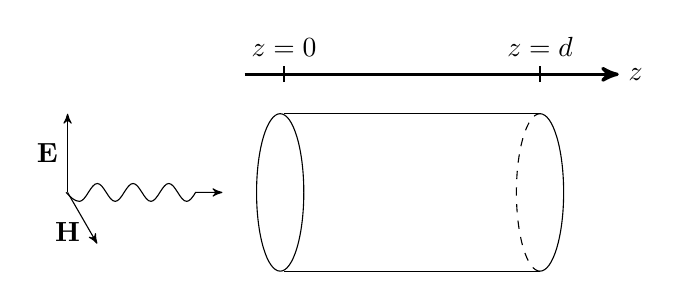
\begin{tikzpicture}[
	scale=1,
	vector/.style={very thick,->, >=latex},
	axis/.style={very thick, ->, >=stealth'}]
	\draw(0:0) arc(0:360:.3 and 1) ;
	\draw(3,-1) arc(-90:90:.3 and 1) ;
	\draw[dashed](3,-1) arc(-90:-270:.3 and 1) ;
	\draw (-0.250,1)--(3,1);
	\draw (-0.250,-1)--(3,-1);
	\draw[shift={(-3.19,0)},axis,thin,x=0.75ex,y=0.75ex] (1.5,0) sin (3,-1) cos (4,0)sin (5,1) cos (6,0) sin (7,-1) cos (8,0)sin (9,1) cos (10,0) sin (11,-1) cos (12,0)sin (13,1) cos (14,0) sin (15,-1) cos (16,0)--(19,0);
	\draw[shift={(-3,0)},axis,thin] (0,0)--(0,1);
	\draw(-3,0.5) node[left]{$\mathbf{E}$};
	\draw[shift={(-3,0)},axis,thin] (0,0)--(-60:.75);
	\draw(-3,-0.5) node[]{$\mathbf{H}$};
	\draw[axis] (-0.75,1.5)--(4,1.5);
	\draw (4,1.5) node [right]{$z$};
	\draw[thick] (-0.25,1.4)--(-0.25,1.6) node[above]{$z=0$};
	\draw[thick] (3,1.4)--(3,1.6) node[above]{$z=d$};

\end{tikzpicture}
\caption{The ol' lossy bar.}
\end{figure}
\subitem{\bf\large (a)} Do this by evaluating the Poynting vector \[\mathbf{P}= \frac{1}{2}\Re e[\mathbf{E}\times\mathbf{H}^*]\] at the two cross-sectional interfaces, then take the difference in real power. (i.e. enforce conservation of energy.)
\begin{IEEEeqnarray*}{lrCl}
\comm{E-field}&\mathbf{E}(z)&=&\hat x E_0 e^{-\alpha z}e^{-j\beta z}\\
\comm{H-field}&\mathbf{H}(z)&=&\frac{1}{\eta}\hat z \times \mathbf{E}\\
&&=&E_0\frac{(\beta-j\alpha)}{\mu\omega}\hat y\\
\comm{since material impedance}&\eta&=&\frac{\omega\mu}{k}=\frac{\omega\mu}{\beta-j\alpha}\\
\comm{power-area density}&\mathbf{P}&=& \frac{1}{2}\Re e[\mathbf{E}\times\mathbf{H}^*]\\
&\mathbf{E}\times\mathbf{H}^*&=&\hat zE_0^2 e^{-\alpha z}e^{-j\beta z}\frac{1}{\eta^*}e^{-\alpha z}e^{j\beta z}(\hat x \times \hat y)\\
&&=&\frac{E_0^2}{\eta^*}e^{-2\alpha z}\\
&\mathbf{P}&=&\frac{1}{2}\Re e\left[\frac{E_0^2}{\eta^*}e^{-2\alpha z}\right]\\
&&=&\frac{1}{2}\Re e\left[E_0^2\frac{(\beta+j\alpha)}{\mu\omega}e^{-2\alpha z}\right]\\
&&=&\frac{1}{2}E_0^2\frac{\beta}{\mu\omega}e^{-2\alpha z}\\
&&=&\omega\sqrt{\frac{\mu\epsilon}{2}}\left[\sqrt{1+\left(\frac{\sigma}{\omega\epsilon}\right)^2}+1\right]^{1/2}\frac{E_0^2}{2\mu\omega}e^{-2\alpha z}\\
&&=&\frac{E_0^2}{2}\sqrt{\frac{\epsilon}{2\mu}}\left[\sqrt{1+\left(\frac{\sigma}{\omega\epsilon}\right)^2}+1\right]^{1/2}e^{-2\alpha z}\\
\comm{interface 1 power} &P_1&=&\frac{E_0^2A}{2}\sqrt{\frac{\epsilon}{2\mu}}\left[\sqrt{1+\left(\frac{\sigma}{\omega\epsilon}\right)^2}+1\right]^{1/2}\\
\comm{interface 2 power} &P_{z=d}&=&\frac{E_0^2A}{2}\sqrt{\frac{\epsilon}{2\mu}}\left[\sqrt{1+\left(\frac{\sigma}{\omega\epsilon}\right)^2}+1\right]^{1/2}e^{-2\alpha d}\\
\comm{real power difference}& P_{absorbed}&=&\frac{E_0^2A}{2}\sqrt{\frac{\epsilon}{2\mu}}\left[\sqrt{1+\left(\frac{\sigma}{\omega\epsilon}\right)^2}+1\right]^{1/2}(1-e^{-2\alpha d})\\ 
\end{IEEEeqnarray*}
\[\boxed{P_{absorbed}=\frac{E_0^2A}{2}\sqrt{\frac{\epsilon}{2\mu}}\left[\sqrt{1+\left(\frac{\sigma}{\omega\epsilon}\right)^2}+1\right]^{1/2}(1-e^{-2\alpha d}) }\]
\subitem{\bf\large (b)} Confirm this result by directly calculating the power absorbed due to conductivity, as typically calculated by \[\frac{1}{2}\int_V\sigma|\mathbf{E}|^2\ud v.\]
Remember, V is the volume of the cylinder of material, and $|\mathbf{E}|^2=\mathbf{E}\cdot\mathbf{E}^*$.
\begin{IEEEeqnarray*}{lrCl}
	\comm{take conjugate}	&\mathbf{E}\cdot\mathbf{E}^*&=	& E_0 e^{-\alpha z}e^{-j\beta z}E_0 e^{-\alpha z}e^{j\beta z}(\hat x\cdot 	\hat x )	\\
	\comm{}	&	&=&E_0^2 e^{-2\alpha z}	\\
	\comm{integral}	&	P_{absorbed}&=&	\frac{1}{2}\int_V\sigma|\mathbf{E}|^2\ud v	\\
	\comm{     }	&	&=&	\frac{E_0^2 \sigma\text{A}}{2}\int_0^de^{-2\alpha z}\ud z	\\
	\comm{     }	&	&=&		-\frac{E_0^2 \sigma\text{A}}{4\alpha}(1-e^{-2\alpha d})\\
\end{IEEEeqnarray*}
\[\boxed{P_{absorb}=-\frac{E_0^2 \sigma\text{A}}{4\alpha}(1-e^{-2d\alpha})}\]

\begin{IEEEeqnarray*}{lrCl}
	\comm{can we show}	&	-\frac{E_0^2 \sigma\text{A}}{4\alpha}&=&P_{absorbed}= \frac{E_0^2A}{2}\sqrt{\frac{\epsilon}{2\mu}}\left[\sqrt{1+\left(\frac{\sigma}{\omega\epsilon}\right)^2}+1\right]^{1/2}\\
	&	-\frac{ \sigma}{2}\sqrt{\frac{2\mu}{\epsilon}}&=&\left[\sqrt{1+\left(\frac{\sigma}{\omega\epsilon}\right)^2}+1\right]^{1/2}\alpha\\
	&	-\frac{ \sigma}{2}\sqrt{\frac{2\mu}{\epsilon}}&=&\left[\sqrt{1+\left(\frac{\sigma}{\omega\epsilon}\right)^2}+1\right]^{1/2}\omega\sqrt{\frac{\mu\epsilon}{2}}\left[\sqrt{1+\left(\frac{\sigma}{\omega\epsilon}\right)^2}-1\right]^{1/2}\\
	&	-\frac{ \sigma}{2\omega}\sqrt{\frac{2\mu}{\epsilon}}\sqrt{\frac{2}{\mu\epsilon}}&=&\left[\sqrt{1+\left(\frac{\sigma}{\omega\epsilon}\right)^2}+1\right]^{1/2}\left[\sqrt{1+\left(\frac{\sigma}{\omega\epsilon}\right)^2}-1\right]^{1/2}\\
	&	-\frac{ \sigma}{\omega\epsilon}&=&\left[\sqrt{1+\left(\frac{\sigma}{\omega\epsilon}\right)^2}+1\right]^{1/2}\left[\sqrt{1+\left(\frac{\sigma}{\omega\epsilon}\right)^2}-1\right]^{1/2}\\
	&	-\frac{ \sigma}{\omega\epsilon}&=&\left[\left(1+\left(\frac{\sigma}{\omega\epsilon}\right)^2\right)-1\right]^{1/2}\\
&	\left(\frac{ \sigma}{\omega\epsilon}\right)^2&=&\left(1+\left(\frac{\sigma}{\omega\epsilon}\right)^2\right)-1\\
&	\left(\frac{ \sigma}{\omega\epsilon}\right)^2&=&\left(\frac{\sigma}{\omega\epsilon}\right)^2\\
\end{IEEEeqnarray*}
Yes, we can.
\end{enumerate}
\end{spacing}

\end{document}


\begin{IEEEeqnarray*}{rClr}
&=&	&\comm{}\\
&=&	&\comm{}\\
\end{IEEEeqnarray*}
	
















